

\documentclass{report}

\usepackage{graphicx, subfigure}
\usepackage{mathtools}
\usepackage{hyperref}
\usepackage{float}
\usepackage[section]{placeins}
\usepackage{listings}

\lstset{frame=tb,
    language=Python,
    basicstyle={\small\ttfamily},
    breaklines=true,
    breakatwhitespace=true,
    tabsize=3
}

\begin{document}
    \title{Monte Carlo Simulations}
    \author{Bruce Berry}
    \maketitle

    \section{Introduction}
    This report details the implementation of various Monte Carlo Techniques for phase separation in metallic solutions.  Grain growth is observed for various material properties under different environments.

    \section{Background}
    The Monte Carlo method is a stochastic approach to evolving systems that uses a set of rules and random selection to simulate species interaction.  Two distinct approaches are employed.

    \subsection{Ising}
    In the Ising approach, a lattice of particles in generated and randomly seeded with initial binary "spin" states, representing the phase of each lattice site.  A random particle is selected and has its spin state flipped. An energy metric is used to decide whether or not to accept the change in spin.  In the experiments presented here, this energy metric is:

    \begin{equation} \label{ising_energy}
        E = \frac{-J}{2} \sum_{i} \sum_{j\ne i} S_i S_j - H \sum_{i} S_i
    \end{equation}
    In \eqref{ising_energy} , the first summation represents particle-particle interaction, while the second summation accounts for an external field applied to the lattice, typically magnetic. A reduction in system energy as a result of the trial is always accepted.  In the case of an increase in energy, the Metropolis algorithm is used to decide on acceptance:
    %
    % \begin{equation} \label{metropolis}
    %     \substack{
    %     W(m \to n) = \exp{\frac{-E_{nm}}{kT}} (E_{nm} \gt 0) \\
    %     W(m \to n) = 1                      (E_{nm} \gt 0)
    %     }
    % \end{equation}

    In the above approach, no attempt is made to conserve the quantity of each spin.  One method of conserving the phase is by adding a term to the energy equation to punish deviations from the initial total concentration.  This results in the modified Ising-alloy method.  The energy equation becomes:

    \begin{equation} \label{ising-alloy_energy}
        E = \frac{-J}{2} \sum_{i} \sum_{j\ne i} s_i s_j + A(\sum_{i} s_{up} - \overline{s_{up}} )^2
    \end{equation}

    \subsection{Q-state Potts Model}
    Generalizing the spin state as in the Ising approach from a binary choice to N states allows parameters such as grain orientations to be simulated.  The Potts method assigns an integer between 1 and N, the Q-state, to each lattice site.  A random nearest neighbor's Q-state is assigned to an initially selected random site.  The energy of each configuration is calculated according to:

    \begin{equation} \label{potts_energy}
        E = \frac{-J}{2} \sum_{i} \sum_{j \ne i} (\delta_{S_i S_j} - 1)
    \end{equation}

    Of interest is the fact that a neighbor only contributes energy to the lattice site if the Q-states are not equal.  Acceptance of the change is decided using the normal Metropolis criteria.

    \section{Methods}
    Simulations were carried out in Python using the numpy numerical library for data structures and generic functions, and matplotlib for plotting. The following parameter studies were performed:
        \begin{itemize}
            \item{Standard Ising model simulation of 500 cycles with all permutations of:}
                \begin{enumerate}
                    \item{kT = 1.5, 0.8, 0.4, 0.1}
                    \item{M = 0.0, 0.5}
                    \item{J = 0.4}
                \end{enumerate}

            \item{Binary Conserved Ising simulation of 500 cycles with paramaterization:}
            \begin{enumerate}
                \item{X$_A$ = 0.3, 0.5}
                \item{kT = 1.5, 0.1}
                \item{J = 0.4, -0.4}
            \end{enumerate}

            \item{Q-State Model simulation of 500 cycles:}
            \begin{enumerate}
                \item{Number of Q-states = 10}
                \item{J = 0.4}
                \item{kT = 0.1}
            \end{enumerate}
        \end{itemize}

    \section{Results}


        \begin{figure}[!htb]
            \label{fig:initial}
            \centering
            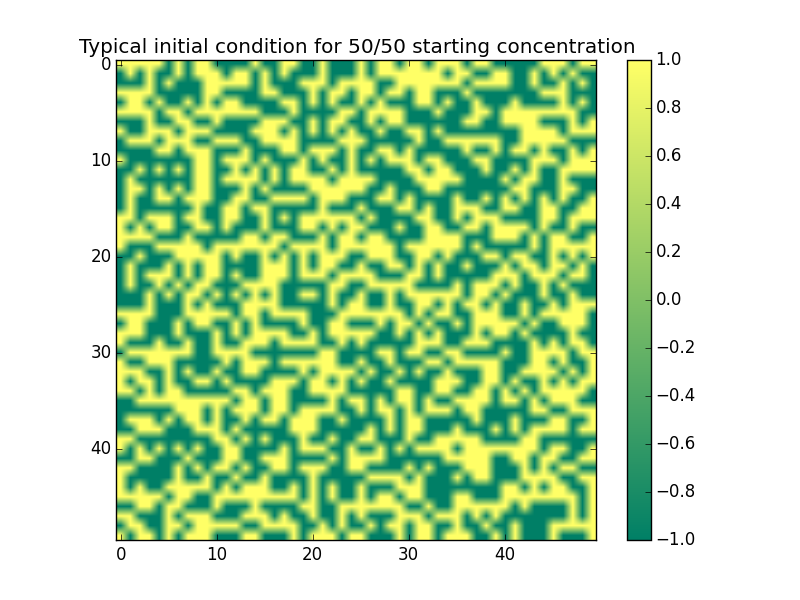
\includegraphics[width=0.4\textwidth]{Initial.png}
            \caption{A representative Initial Condition.}
        \end{figure}

        \begin{figure}[!htb]
            \label{fig:Ising}
            \subfigure[] {
            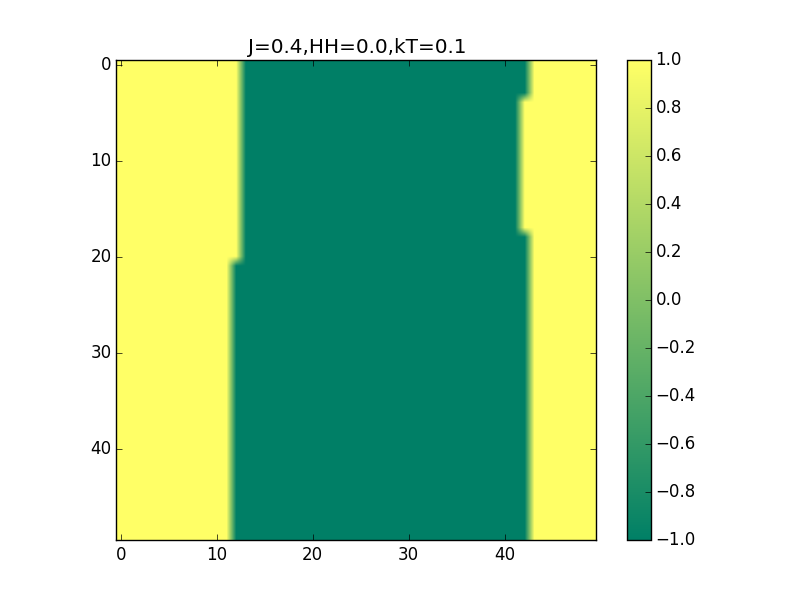
\includegraphics[width=0.6\textwidth]{J04-HH0-kT1.png}
            }
            \subfigure[] {
            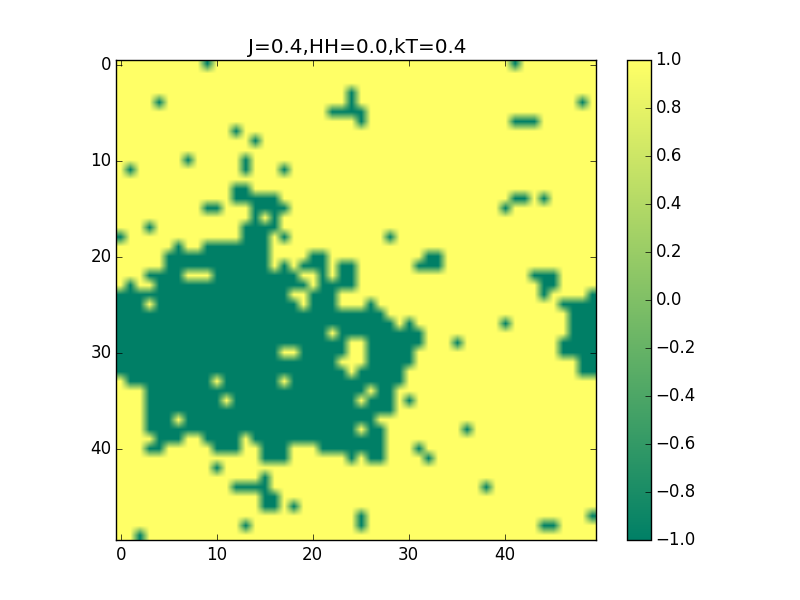
\includegraphics[width=0.6\textwidth]{J04-HH0-kT4.png}
            }
            \subfigure[] {
            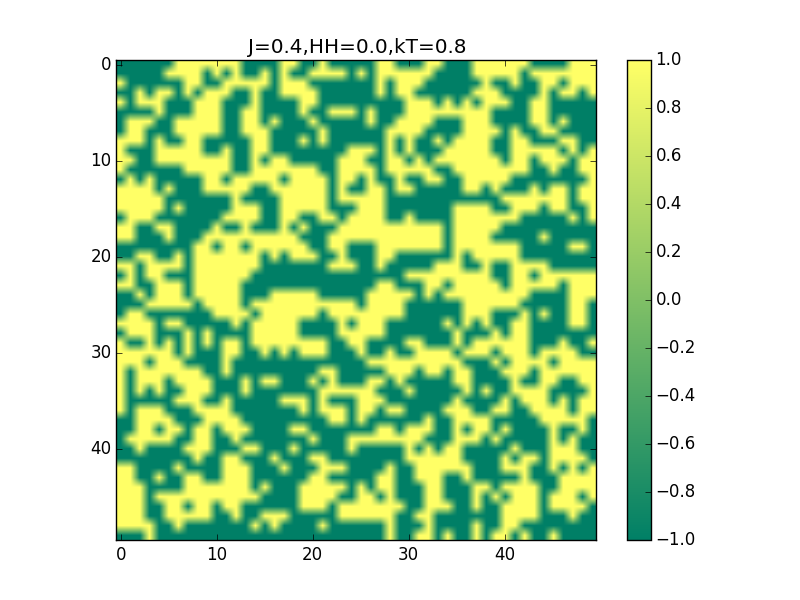
\includegraphics[width=0.6\textwidth]{J04-HH0-kT8.png}
            }
            \subfigure[] {
            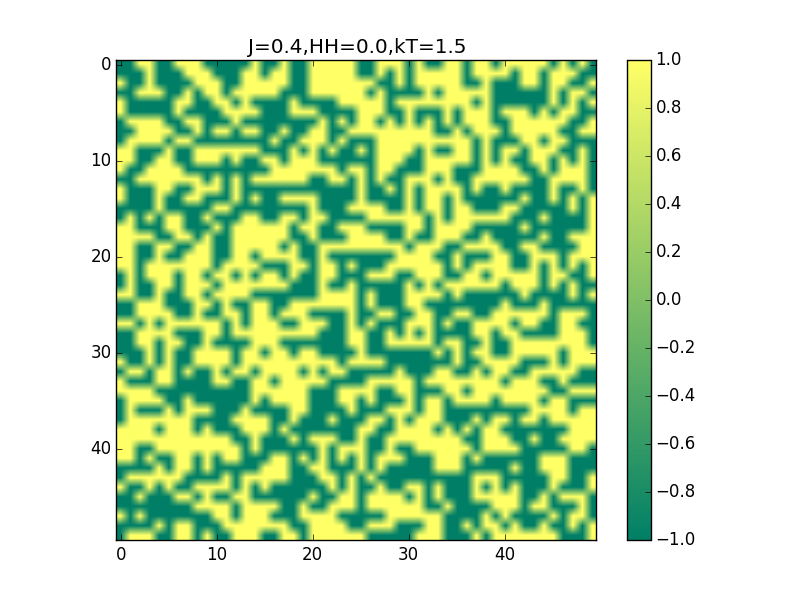
\includegraphics[width=0.6\textwidth]{J04-HH0-kT15.png}
            }
            \caption{Final state for all temperatures with no magnetic field applied.
            A decrease in the temperature parameter results in a higher incidence
            of "clumping".}
        \end{figure}

        \begin{figure}[!htb]
            \label{fig:Ising-mag}
            \subfigure[] {
            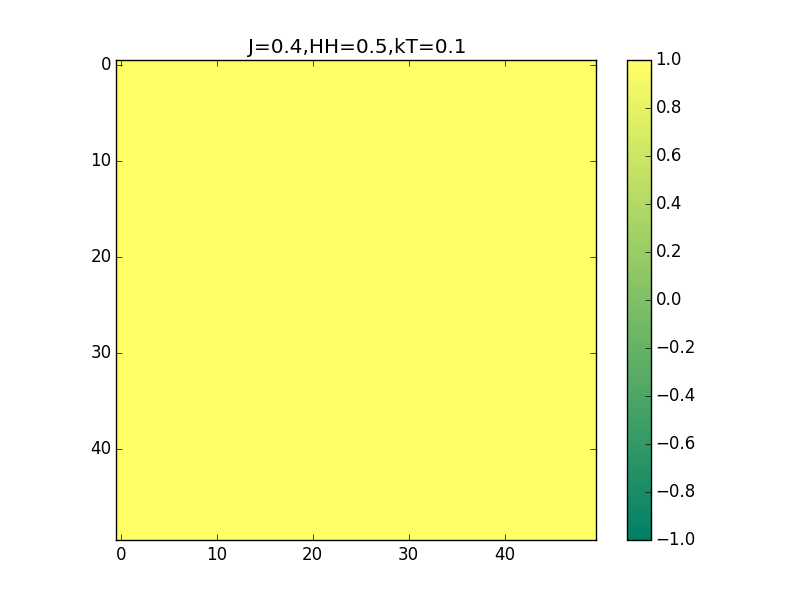
\includegraphics[width=0.6\textwidth]{J04-HH5-kT1.png}
            }
            \subfigure[] {
            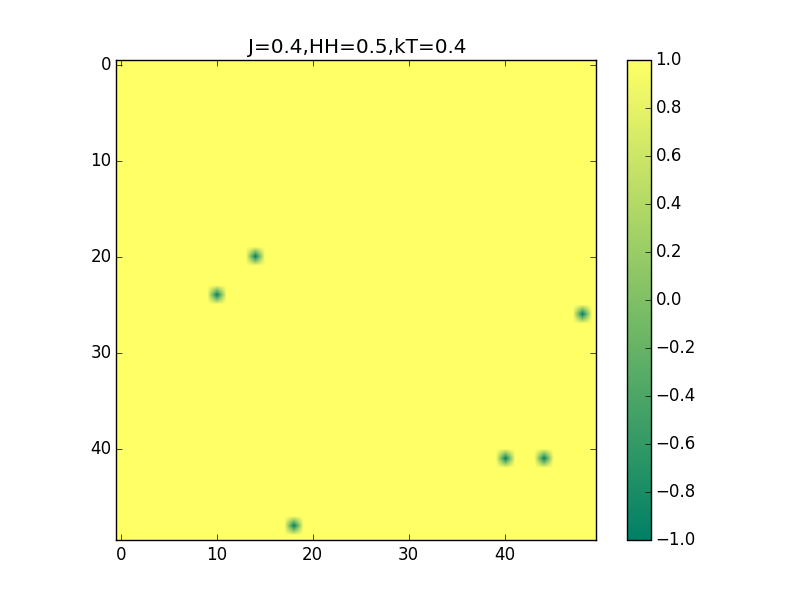
\includegraphics[width=0.6\textwidth]{J04-HH5-kT4.png}
            }
            \subfigure[] {
            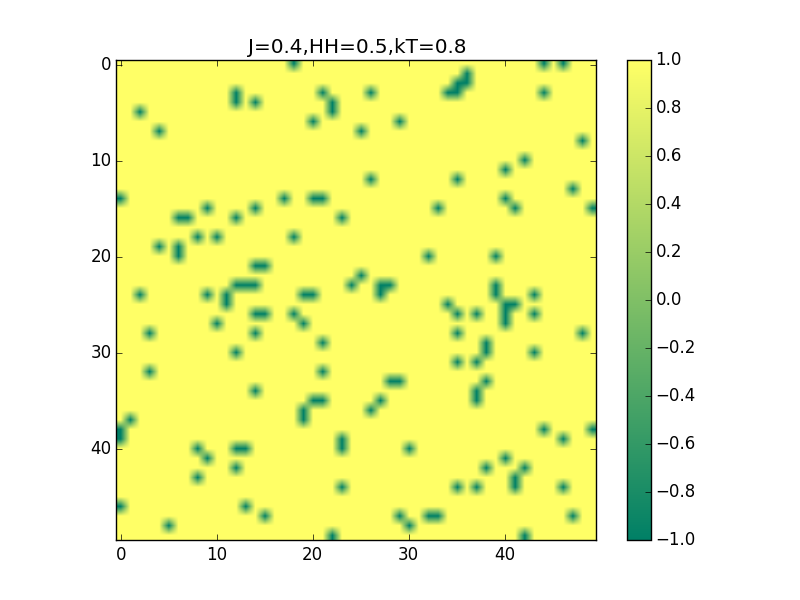
\includegraphics[width=0.6\textwidth]{J04-HH5-kT8.png}
            }
            \subfigure[] {
            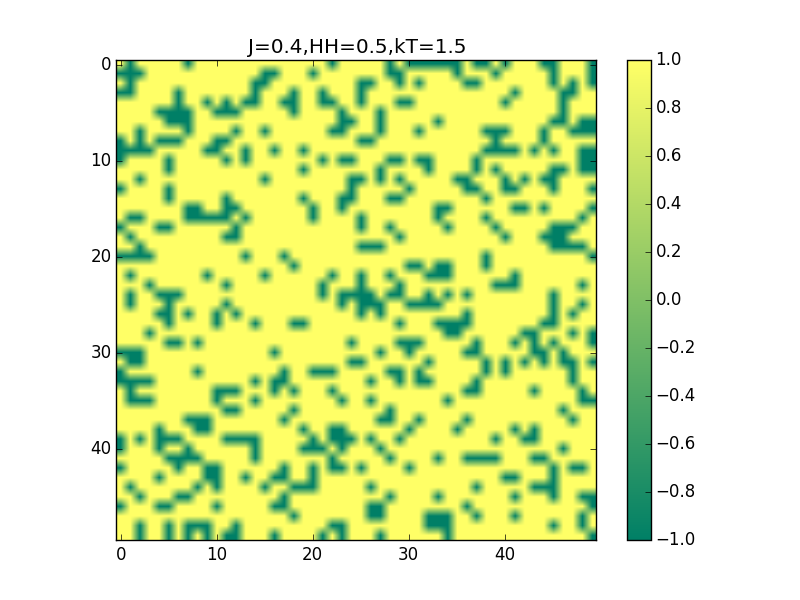
\includegraphics[width=0.6\textwidth]{J04-HH5-kT15.png}
            }
            \caption{Final state for all temperatures with magnetic field applied.}
        \end{figure}


        \begin{figure}[!htb]
            \label{fig:Ising-alloy-0.3}
            \subfigure[] {
            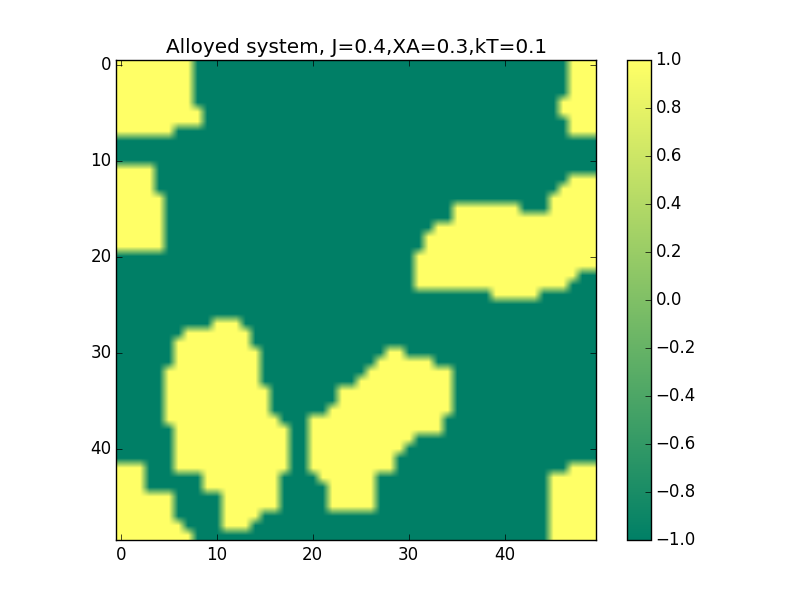
\includegraphics[width=0.6\textwidth]{Alloy-A3-kT1-J4.png}
            }
            \subfigure[] {
            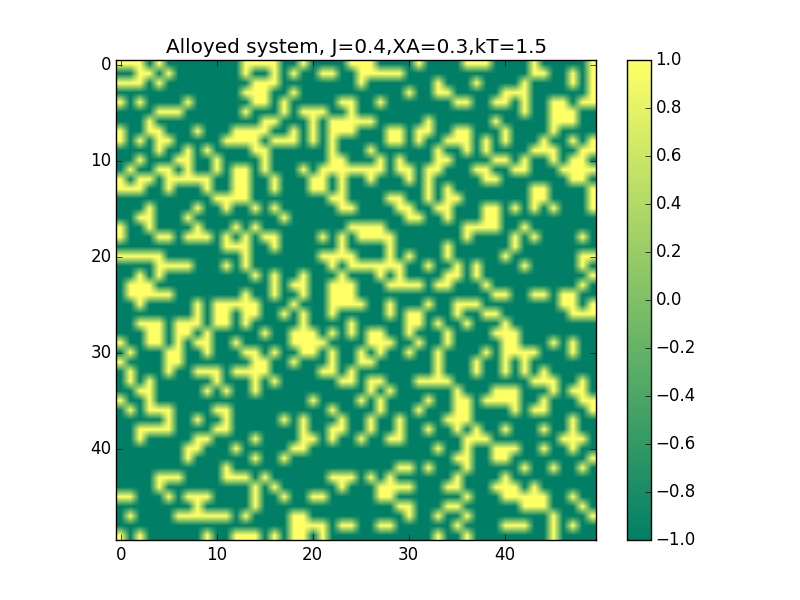
\includegraphics[width=0.6\textwidth]{Alloy-A3-kT15-J4.png}
            }
            \subfigure[] {
            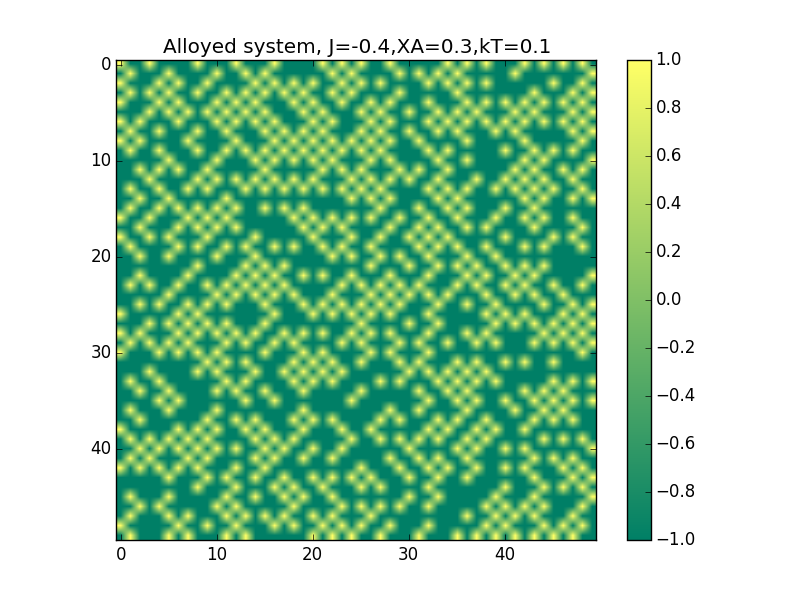
\includegraphics[width=0.6\textwidth]{Alloy-A3-kT1-J4neg.png}
            }
            \subfigure[] {
            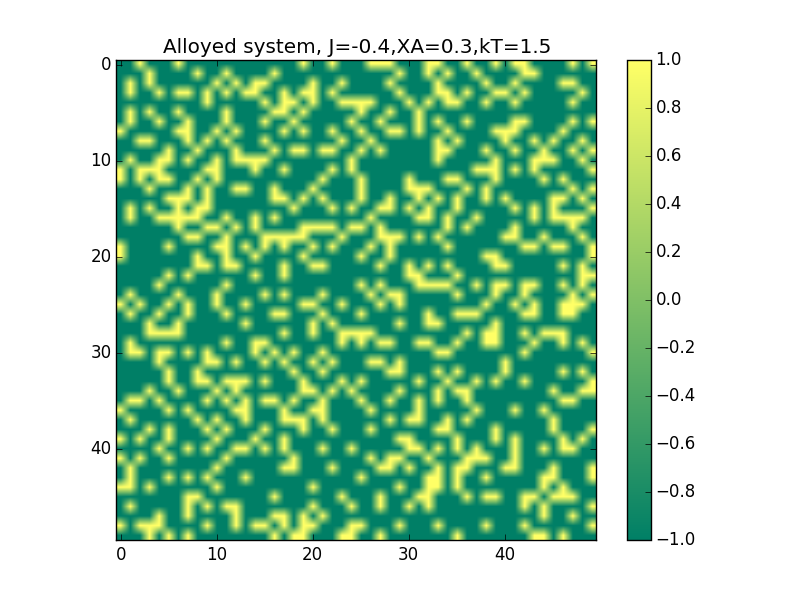
\includegraphics[width=0.6\textwidth]{Alloy-A3-kT15-J4neg.png}
            }
            \caption{Final state for initial $X_A = 0.3$. (a) and (b) vary temperature for positive J, (c), (d) for negative J.}
        \end{figure}


        \begin{figure}[!htb]
            \label{fig:Ising-alloy-0.5}
            \subfigure[] {
            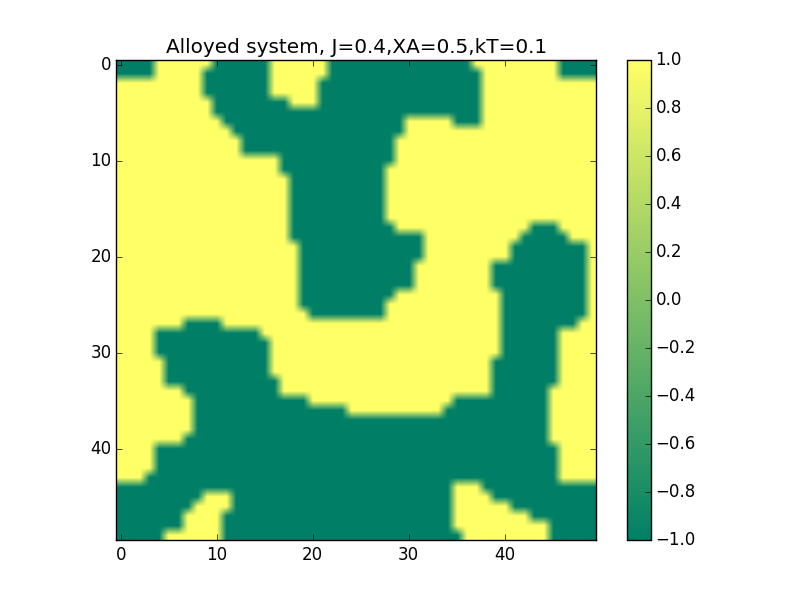
\includegraphics[width=0.6\textwidth]{Alloy-A5-kT1-J4.png}
            }
            \subfigure[] {
            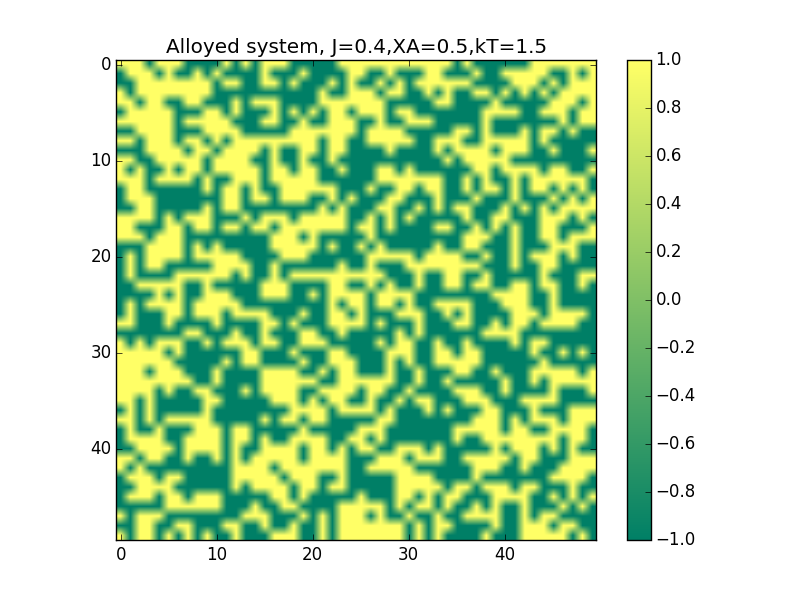
\includegraphics[width=0.6\textwidth]{Alloy-A5-kT15-J4.png}
            }
            \subfigure[] {
            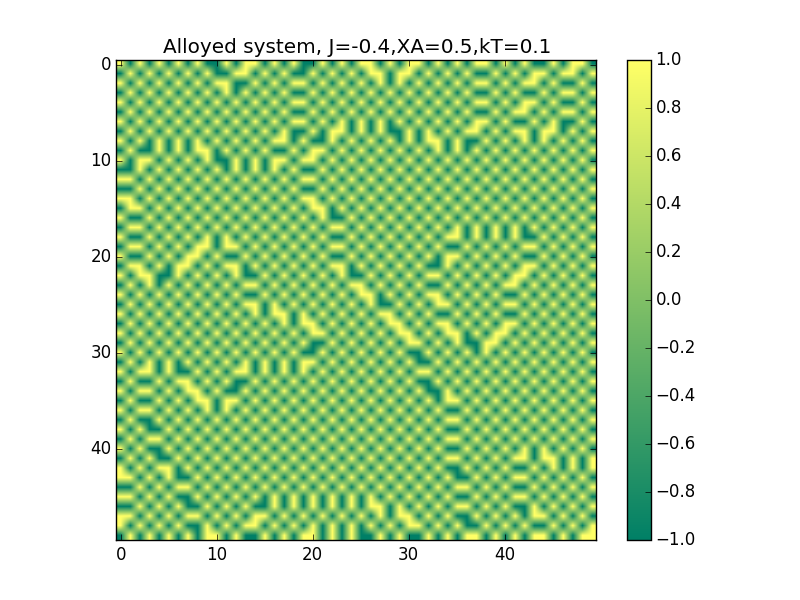
\includegraphics[width=0.6\textwidth]{Alloy-A5-kT1-J4neg.png}
            }
            \subfigure[] {
            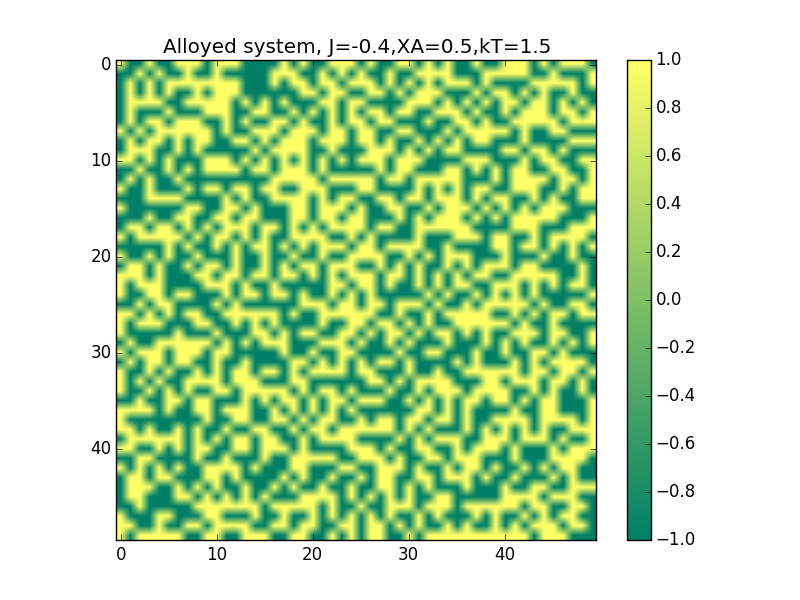
\includegraphics[width=0.6\textwidth]{Alloy-A5-kT15-J4neg.png}
            }
            \caption{Final state for initial $X_A = 0.5$. (a) and (b) vary temperature for positive J, (c), (d) for negative J.}
        \end{figure}

        \begin{figure}[!htb]
            \label{fig:Potts}
            \subfigure[] {
            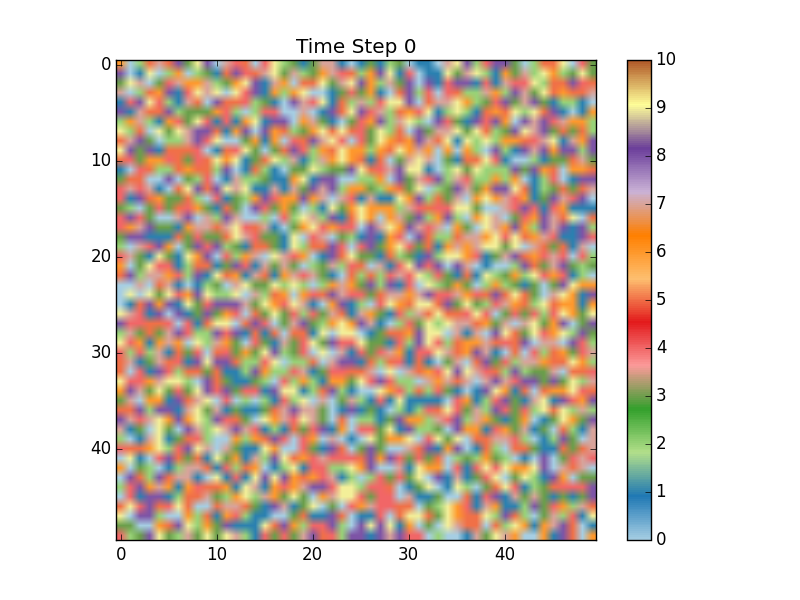
\includegraphics[width=0.6\textwidth]{Potts0.png}
            }
            \subfigure[] {
            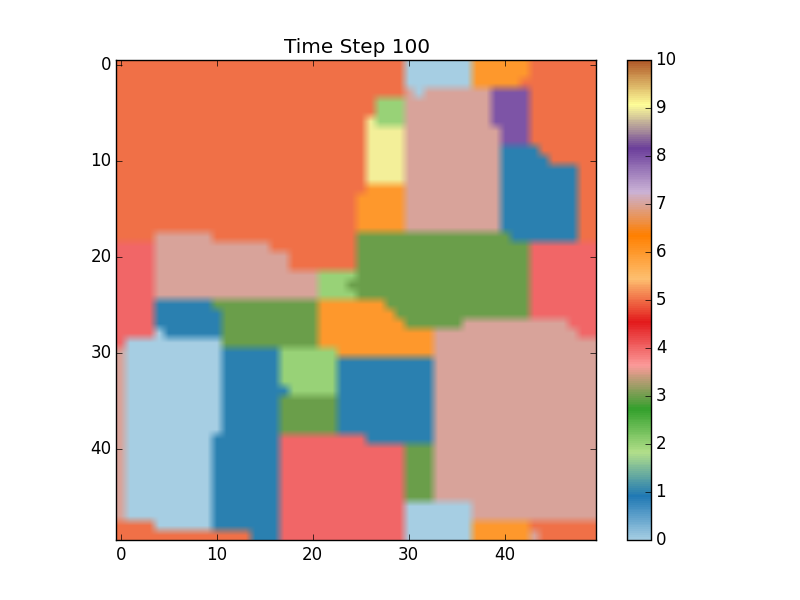
\includegraphics[width=0.6\textwidth]{Potts100.png}
            }
            \subfigure[] {
            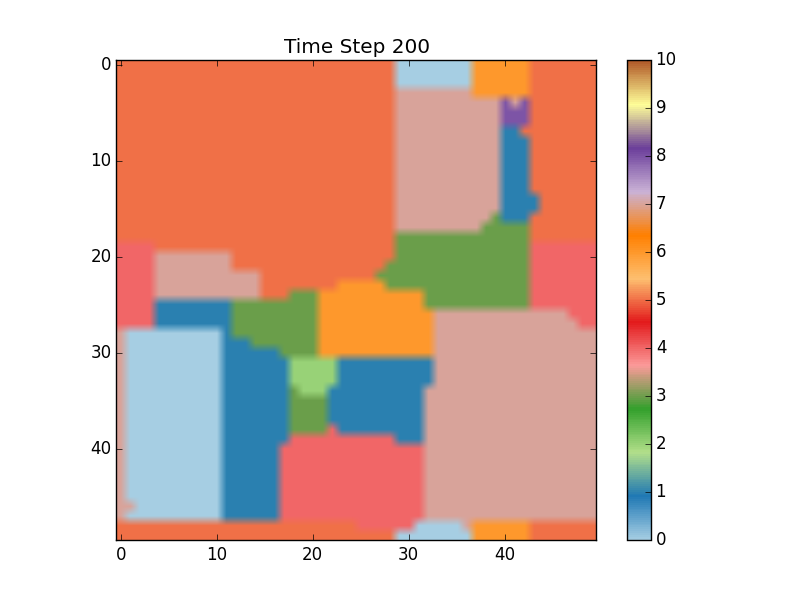
\includegraphics[width=0.6\textwidth]{Potts200.png}
            }
            \subfigure[] {
            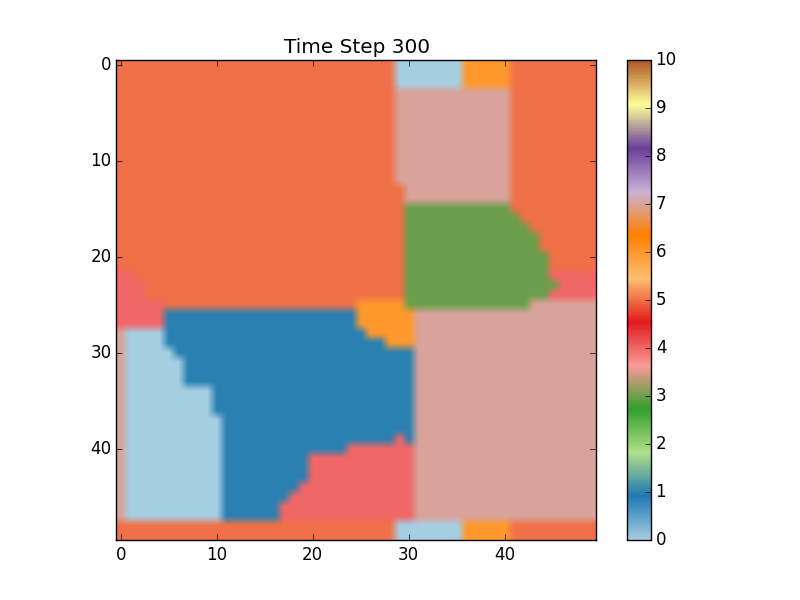
\includegraphics[width=0.6\textwidth]{Potts300.png}
            }
            \caption{Potts evolution for Q=10.  Grain growth is evident in initial stages and progresses to dominance of one grain throughout domain.}
        \end{figure}

    \section{Discussion}
    \subsection{Part A}
        A decrease in temperature raises the incidence of clumping when no magnetic field is applied.  This is a result of the system attempting to minimize energy.  In effect, A-A bonds become favorable to A-B bonds as the system approaches the "solvus" line. With an applied magnetic field, the second part of \eqref{ising_energy} can contribute to the total energy, such that an increase in temperature can result in a spin flip to occur.
    \subsection{Part B}
        Non-strict conservation of the spin totals at low temperatures encourages smooth interfaces with few A-B bonds.  This behavior can be overcome by an increase in temperature, effectively using enthalpy to overcome entropy.  When negating the diffusion coefficient, J, ordered systems become common for moderatly low temperatures.  This suggests that A-B bonds are energetically favorable to A-A or B-B bonds. Greatly increasing the temperature shifts the energy balance such that both bond types can exist, resulting in comparatively unordered states.
    \subsection{Part C}
        The initial grain structure is highly random, making early switch attempts very energeticly favorable.  This has the affect of causing the simulation to progress rapidly in the early time steps.  As grain boundaries begin to emerge and the interface "area" decreases, sites less likely to exist on a grain boundary, slowing the simulation.  Regardless of the slowdown, grain growth is evident when comparing snapshots from t=0 to 300.  An interesting simulation artifact is noticed when kT is increased to a large value, say 1.5.  In this case, a spin change becomes unrealisticly favorable, causing spattering of grain boundaries in an unpredicable manner, as shown in \ref{fig:high_temp} in the Appendix. This could be interpreted as a breakdown in the validity of the Potts model due to the assumptions made in the behavior with respect to temperature, such as partial of complete melting of the lattice.

        Also of interest is the fact that the results seem highly dependent on the initial random seed. A common result is early dominance of only one or two grains.  An example has not been given here.





    \section{Appendix}
    \begin{figure}[!htb]
        \label{fig:high_temp}
        \subfigure[] {
        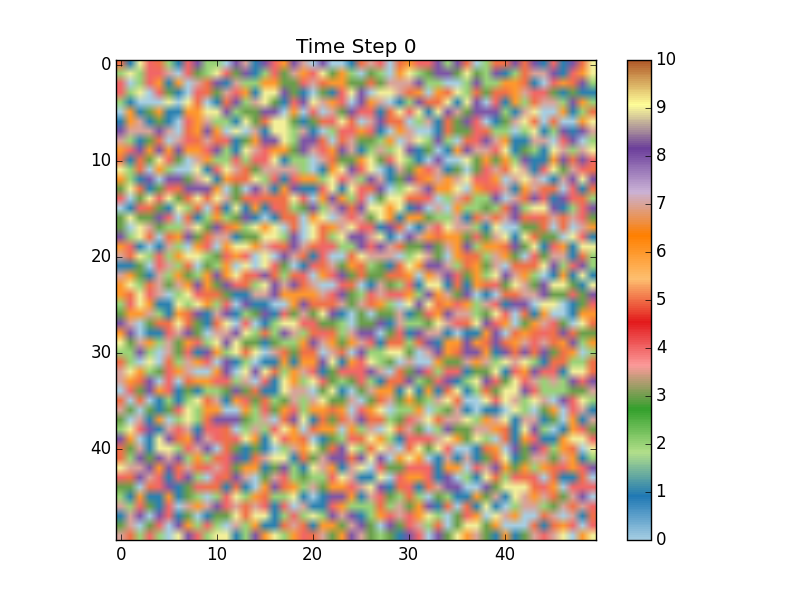
\includegraphics[width=0.6\textwidth]{Potts0_high.png}
        }
        \subfigure[] {
        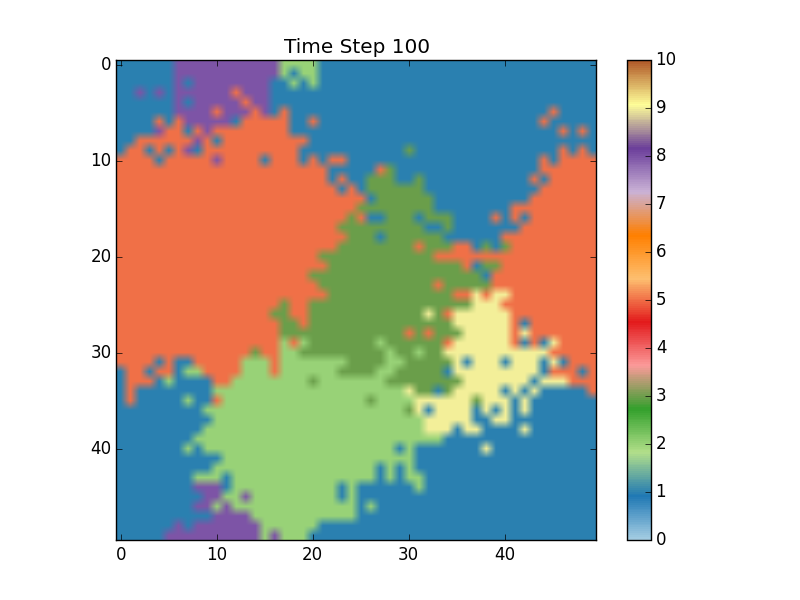
\includegraphics[width=0.6\textwidth]{Potts100_high.png}
        }
        \subfigure[] {
        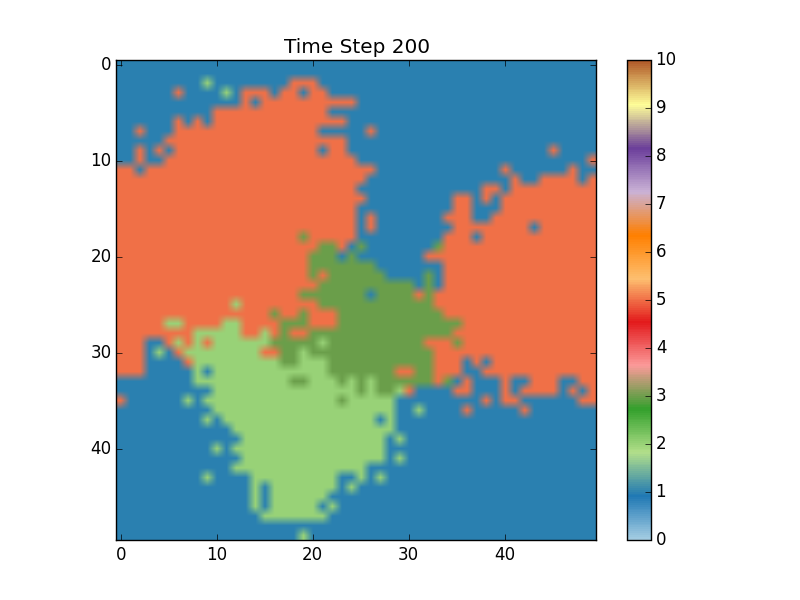
\includegraphics[width=0.6\textwidth]{Potts200_high.png}
        }
        \subfigure[] {
        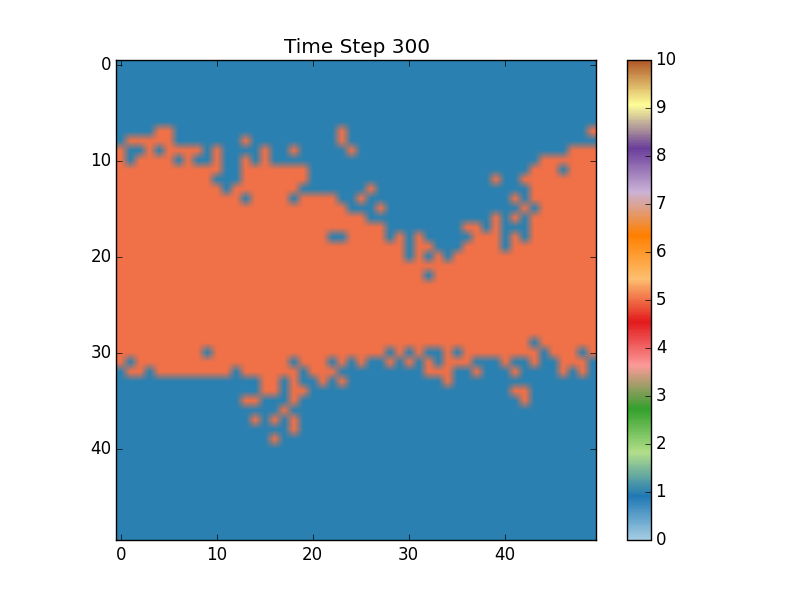
\includegraphics[width=0.6\textwidth]{Potts300_high.png}
        }
        \caption{Grain growth at high temperature kT = 1.5. Apparent jumping of grains deep into the center of another grain is observed.}
    \end{figure}


    \subsection{Sourcecode}
    Sourcecode has been attached seperately for readability.


\end{document}
